% Copyright 2026 Sreeram Anil
% SPDX-License-Identifier: CC-BY-4.0
% =============================================================================
%  Real-time-iteration moving-horizon estimation (MHE-RTI)
% =============================================================================
\chapter{Real-time-iteration moving-horizon estimation (MHE-RTI)}
\label{ch:mherti}

\section*{At a glance}
\begin{tabular}{@{}l>{\raggedright\arraybackslash}p{0.76\textwidth}@{}}
Family & optimization (moving horizon) \\
Header & \texttt{include/estkit/optimization/mhe.hpp} (\texttt{max\_iter = 1}) \\
Registered name & \texttt{MHE-RTI} \\
State dimension & $n_x = 4$ (cell model) --- generic in $n_x,n_u,n_y$; horizon $N = 20$ \\
Decision variables & $(N{+}1)n_x = 84$, solved by \emph{one} Gauss--Newton step per sample \\
Cost per step & exactly one assemble--factor--solve, $\mathcal{O}(N n_x^3)$;
measured \SI{17}{\micro\second}, data-independent \\
Memory & \SI{26.9}{\kilo\byte} fixed arrays \\
Primary references & \cite{diehl2005rti,kuhl2011rtimhe,rao2003mhe,rawlings2017mpc} \\
\end{tabular}

\section{Motivation and aerospace/BMS relevance}
The estimator of Chapter~\ref{ch:mhe} solves a nonlinear program at every sampling instant.  For an
avionics task that is not merely expensive, it is \emph{structurally} awkward: the number of
Gauss--Newton iterations depends on the data, so the execution time depends on the data, so the
worst-case execution time has to be bounded by the iteration cap rather than by the typical
behaviour, and the task must be budgeted for a case that almost never occurs.  Iterative solvers
sit badly inside a fixed-period control loop.

\citet{diehl2005rti} observed that the iteration does not have to converge at every instant,
because the problem solved at instant $k{+}1$ is a small perturbation of the one solved at $k$: the
window has moved by one sample, so the solution manifold has moved by $\mathcal{O}(\dt)$.  If the
previous solution is shifted forward and used as the initial guess, a \emph{single} Newton-type
iteration lands within $\mathcal{O}(\dt^2)$ of the new solution; repeating this at every instant,
the iterates \emph{track} the solution manifold instead of converging to a point on it at every
step.  This is the real-time iteration (RTI) scheme.  \citet{kuhl2011rtimhe} carried it over from
optimal control to moving-horizon state and parameter estimation, which is the form used here.

The practical consequence is what matters for an aircraft battery management computer: the cost per
sample becomes a \emph{constant}, known at design time --- one Jacobian assembly, one
block-tridiagonal factorisation, one back-substitution --- with no data-dependent loop and no
convergence test.  Worst-case execution time equals typical execution time.  In exchange, the
estimate at any instant is a first-order-accurate tracking of the optimum rather than the optimum
itself, and this chapter measures what that costs.

\section{Problem statement and assumptions}
The nonlinear program, the arrival cost, the constraint set and the Gauss--Newton normal equations
are exactly those of Chapter~\ref{ch:mhe}, \crefrange{eq:mhe-nlp}{eq:mhe-proj}; they are not
repeated.  What changes is the termination rule and one additional assumption.

\begin{assumption}[Contraction and shift]\label{as:rti-contract}
The Gauss--Newton iteration applied to \cref{eq:mhe-nlp} is locally contractive with rate
$\kappa < 1$ in a neighbourhood of the solution manifold, and the shifted previous solution lies
inside that neighbourhood.
\end{assumption}

Assumption~\ref{as:rti-contract} is where the method is either safe or not.  Gauss--Newton is
contractive when the residual at the solution is small relative to the curvature of the residual
map --- the classical small-residual condition \citep[\S10.3]{nocedal2006}.  For the cell model the
only nonlinearity in the state is the open-circuit-voltage curve $\ocv(\soc)$, whose second
derivative is bounded by roughly \SI{20}{\volt} per unit SOC squared on this NMC chemistry, and the
residual at the solution is the sensor noise, a few millivolts.  The product is small, $\kappa$ is
of order $10^{-2}$, and a single iteration removes almost all of the error the shift introduced.

\section{Derivation}

\subsection{Shift-and-append warm start}
Let $\mathcal{X}^\star_k = (\vx^\star_0,\dots,\vx^\star_N)$ be the iterate held after the update at
instant $k$, node $j$ corresponding to absolute time $k-N+j$.  At instant $k{+}1$ the window covers
$[k-N+1,\,k+1]$, so the warm start is obtained by discarding the oldest node, shifting, and
appending one model step:
\begin{equation}\label{eq:rti-shift}
\vx^{(0)}_j = \vx^\star_{j+1},\quad j = 0,\dots,N-1,
\qquad
\vx^{(0)}_N = f\bigl(\vx^\star_N,\ \vu_k\bigr).
\end{equation}
Simultaneously the arrival cost is advanced past the discarded node by
\crefrange{eq:mhe-arrS}{eq:mhe-arrx}.  The nodes $0,\dots,N-1$ of \cref{eq:rti-shift} are already
optimal for the \emph{previous} problem; they are not optimal for the new one only because the new
measurement $\vy_{k+1}$ has arrived and the arrival cost has moved by one sample.  Both are
$\mathcal{O}(1)$ perturbations of a \emph{single} residual block out of $2N{+}2$, which is why the
warm start is good.

\subsection{One iteration, and what it costs}
Let $\mathcal{X}^\star(k)$ denote the exact minimiser at instant $k$ and define the tracking error
$e_k = \norm{\mathcal{X}^{(0)}_k - \mathcal{X}^\star(k)}$ of the warm start and
$\varepsilon_k = \norm{\mathcal{X}^{\text{RTI}}_k - \mathcal{X}^\star(k)}$ of the single-iteration
result.  Local contraction gives
\begin{equation}\label{eq:rti-contract}
\varepsilon_k \le \kappa\, e_k + \mathcal{O}(e_k^2),
\qquad
e_{k+1} \le \varepsilon_k + \Delta_k,
\end{equation}
where $\Delta_k$ is the displacement of the solution manifold between two instants, i.e.\ the
effect of adding one measurement and removing one.  Combining, the tracking error obeys the
linear recursion $\varepsilon_{k+1}\le \kappa(\varepsilon_k + \Delta_k)$, whose fixed point is
\begin{equation}\label{eq:rti-fixed}
\varepsilon_\infty \le \frac{\kappa}{1-\kappa}\,\sup_k \Delta_k .
\end{equation}
\Cref{eq:rti-fixed} is the whole stability rationale of the scheme, and it says three useful things.
The RTI estimate never converges to the optimum, but it stays within a bounded neighbourhood of it;
the neighbourhood shrinks with the contraction rate $\kappa$, i.e.\ with the smallness of the
residual; and it shrinks with $\Delta_k$, i.e.\ with the sampling interval.  Sampling faster makes
RTI \emph{more} accurate relative to the converged solution, not less --- the opposite of the
intuition one brings from explicit integrators.  A rigorous version of this argument, including the
effect of active-set changes, is given by \citet{diehl2005rti}; \citet{kuhl2011rtimhe} verify it
numerically for moving-horizon estimation.

Two remarks specific to this implementation.  First, the classical RTI splits each iteration into a
\emph{preparation} phase (assemble and factor the KKT matrix using the previous state) and a
\emph{feedback} phase (one back-substitution once the new measurement arrives), so that the latency
between measurement and output is a single triangular solve.  For a state \emph{estimator} with no
control output to deliver, the split buys nothing --- there is no downstream actuator waiting --- so
it is not implemented; the whole iteration runs after the measurement.  It would become worthwhile
if the SOC estimate fed a power-limit computation with a hard latency requirement, and the code is
structured so that the split is a refactoring rather than a redesign.  Second, an active-set change
(the SOC hitting a bound) violates the smoothness underlying \cref{eq:rti-contract}.  The projected
step \cref{eq:mhe-proj} degrades gracefully in that case --- it returns a feasible point --- but the
first-order tracking property is lost for as long as the constraint is switching.

\section{Algorithm}
\begin{algorithm}[H]
\caption{MHE-RTI --- one sampling period (constant cost)}
\begin{algorithmic}[1]
\Require previous window $\{\vx^\star_j,\vu_j,\vy_j\}_{j=0}^{N}$, arrival $(\bar\vx,\Pi)$, filtered
         history $\{\hat\vx_{j|j}\}$, new $\vu_{k-1}$, $\vy_k$, $\vu_k$
\Statex \textbf{Shift} \Comment{constant cost}
\State advance $(\bar\vx,\Pi)$ past node $0$ by \crefrange{eq:mhe-arrS}{eq:mhe-arrx}
\State shift the window and append $\vx_N \gets f(\vx_{N-1},\vu_{k-1})$ \Comment{\cref{eq:rti-shift}}
\State $\vy_N\gets\vy_k$, $\vu_N\gets\vu_k$
\Statex \textbf{Prepare} \Comment{constant cost}
\State $\mQ_j^{-1},\mR_j^{-1}$ at all nodes; $\Pi^{-1}$
\State $\mF_j \gets \partial f/\partial\vx|_{\vx_j,\vu_j}$, $\mH_j \gets \partial h/\partial\vx|_{\vx_j,\vu_j}$
\State $\vw_j \gets \vx_{j+1}-f(\vx_j,\vu_j)$, $\vv_j\gets\vy_j-h(\vx_j,\vu_j)$
\State assemble $\bm{M}_{jj},\mB_j,\bm{g}_j$ by \crefrange{eq:mhe-A}{eq:mhe-g}
\Statex \textbf{Solve (one Gauss--Newton step, no convergence test)}
\State forward sweep $\mD_j,\mL_j,\vz_j$ and back substitution $\delta\vx_j$ \Comment{\cref{eq:mhe-ldl}}
\State $\vx_j \gets \mathcal{P}_{\mathbb{X}}(\vx_j + \delta\vx_j)$ for all $j$ \Comment{\cref{eq:mhe-proj}, $\alpha=1$}
\State record $\hat\vx_{k|k}\gets\vx_N$ for the next arrival-cost update
\Ensure $\hat\vx_k = \vx_N$, $\mP_k = \mD_N^{-1}$ (\cref{prop:mhe-marg})
\end{algorithmic}
\end{algorithm}

Every line has a fixed cost.  There is no loop bound to justify, no tolerance to tune, and no
branch whose outcome depends on the measurement --- except the projection \cref{eq:mhe-proj}, whose
two comparisons per state are constant-time.

\section{Application to the battery model}
The registered instance is the same \texttt{Mhe<EcmModel,20>} class as Chapter~\ref{ch:mhe},
configured with \texttt{max\_iter = 1}, \texttt{backtrack\_max = 0} and the box
$\soc\in[0,1]$, $h\in[-1,1]$.  Nothing else differs: same horizon, same arrival cost (the smoothing
update, for the reasons given in Chapter~\ref{ch:mhe}), same $\mQ$, $\mR$ and Jacobians.  The pair
therefore forms a clean controlled experiment --- the only variable is how many Gauss--Newton steps
are taken per sample --- and the comparison in \cref{sec:rti-results} isolates exactly the RTI
approximation.

With $\dt = \SI{0.1}{\second}$ and $N = 20$ the window spans \SI{2}{\second}.  The shift of
\cref{eq:rti-shift} moves the window by \SI{5}{\percent} of its length per sample; with a cruise
current of about \SI{5.5}{\ampere} the SOC moves by \SI{3e-3}{\percent} between samples, and the RC
voltages by at most \SI{0.1}{\milli\volt}.  The perturbation $\Delta_k$ of \cref{eq:rti-fixed} is
therefore genuinely small, which is the quantitative reason the scheme works here.

\section{Implementation notes}
\paragraph{Where the constant cost comes from.}  Per sample: $2(N{+}1) = 42$ evaluations of $f$ and
$h$, $2N{+}1 = 41$ Jacobian evaluations, $N{+}1 = 21$ inversions of a $4\times4$ $\mQ$ and a scalar
$\mR$, $\approx 6(N{+}1)$ products of $4\times4$ matrices for \crefrange{eq:mhe-A}{eq:mhe-g}, and
$N{+}1$ symmetric $4\times4$ solves in \cref{eq:mhe-ldl}.  That is about $\num{25000}$ flops plus
$\approx 130$ calls to \texttt{exp} (the ECM's Arrhenius and hysteresis coefficients), and the
transcendentals, not the linear algebra, dominate the measured \SI{17}{\micro\second}.  Caching
$a_1(T), a_2(T), a_h(i)$ per node across the assembly would cut the cost by roughly a third and is
the first optimisation to make on an embedded target.

\paragraph{Determinism.}  No dynamic memory, no recursion, no data-dependent iteration count, no
exception path.  The only conditional branches are the projection comparisons and the
\texttt{is\_finite} guard that aborts the sweep if a block factor degenerates --- in which case the
estimator keeps the warm-started iterate, which is a feasible, model-consistent trajectory rather
than a NaN.  This is the fallback behaviour one wants to be able to state in a safety case.

\paragraph{The covariance is free.}  \Cref{prop:mhe-marg} makes $\mD_N^{-1}$, already computed in
the forward sweep, the Gauss--Newton posterior covariance of the current estimate, so \texttt{P()}
and the benchmark's $\pm2\sigma$ band cost nothing extra.  An RTI estimator therefore reports an
uncertainty just as a Kalman filter does --- which is not true of every optimisation-based
estimator.

\paragraph{Smoothed estimates are free too.}  The window holds $\hat\vx_{k-N+j\mid k}$ for all
$j$, i.e.\ a fixed-lag smoother of lag up to \SI{2}{\second}, exposed through \texttt{node(j)}.
Nothing in the benchmark uses it, but for a diagnostic function --- detecting a cell that behaved
anomalously two seconds ago --- it is available at zero cost.

\paragraph{\texttt{float} build.}  Verified against Table~\ref{tab:float}: \texttt{nominal} gives
\SI{0.08}{\percent} in both precisions, \texttt{init\_error} \SI{0.11}{} against
\SI{0.13}{\percent}, \texttt{aged\_cell} \SI{0.79}{} against \SI{0.81}{\percent} and
\texttt{combined} \SI{0.50}{} against \SI{0.55}{\percent} --- the single-precision build is
marginally \emph{better} on three of the four.  The ill-conditioning discussed in
Chapter~\ref{ch:mhe} is structured rather than random, so single precision survives it; a production single-precision implementation should
nevertheless prefer a square-root form of \cref{eq:mhe-ldl}.

\section{Benchmark results}
\label{sec:rti-results}
% Copyright 2026 Sreeram Anil
% SPDX-License-Identifier: CC-BY-4.0
\begin{table}[H]\centering\footnotesize\setlength{\tabcolsep}{4pt}
\caption{MHE-RTI: cell-level benchmark on the eVTOL mission (mean over seeds; RMSE and max error in \% SOC; $t_\mathrm{conv}$: first time the error stays below 2\,\% for 60\,s, -- = never; EKF reference: steady-state RMSE of the plain EKF on the same data).}\label{tab:cell_MHERTI}
\begin{tabular}{llrrrrrcrr}\toprule
plant & scenario & RMSE & RMSE$_\mathrm{ss}$ & max & $t_\mathrm{conv}$ [s] & RMSE$_v$ [mV] & div. & EKF ref. & ns/step \\ \midrule
ECM & nominal & 0.36 & 0.08 & 1.58 & 0 & 0.85 & no & 0.05 & 17270 \\
ECM & init\_error & 0.23 & 0.11 & 1.16 & 0 & 2.14 & no & 0.05 & 17258 \\
ECM & current\_bias & 0.54 & 0.10 & 2.00 & 66 & 0.88 & no & 0.61 & 17292 \\
ECM & noise\_step & 0.99 & 1.23 & 2.32 & 0 & 3.75 & no & 0.12 & 17292 \\
ECM & outliers & 0.88 & 0.70 & 2.89 & 119 & 2.62 & no & 0.21 & 17338 \\
ECM & cold & 0.75 & 0.76 & 1.86 & 0 & 1.93 & no & 0.16 & 17328 \\
ECM & hot & 0.23 & 0.04 & 1.19 & 0 & 0.62 & no & 0.03 & 17277 \\
ECM & aged\_cell & 1.20 & 0.71 & 5.73 & 0 & 3.41 & no & 1.52 & 17230 \\
ECM & param\_mismatch & 2.40 & 2.19 & 5.42 & 0 & 2.71 & no & 1.36 & 17305 \\
ECM & sensor\_dropout & 1.51 & 0.43 & 6.73 & 0 & 2.00 & no & 0.46 & 17244 \\
ECM & preisach & 0.97 & 0.46 & 3.56 & 158 & 0.86 & no & 0.20 & 17252 \\
ECM & combined & 0.74 & 0.50 & 7.36 & 0 & 4.28 & no & 12.44 & 17156 \\
\midrule
SPM & nominal & 4.43 & 4.55 & 5.26 & 0 & 1.02 & no & 3.73 & 16705 \\
SPM & init\_error & 4.17 & 4.28 & 5.12 & 0 & 2.17 & no & 3.81 & 16578 \\
SPM & current\_bias & 5.70 & 6.45 & 7.31 & 0 & 1.09 & no & 5.69 & 16572 \\
SPM & noise\_step & 6.40 & 7.82 & 11.41 & 0 & 3.78 & no & 3.30 & 16686 \\
SPM & outliers & 3.66 & 4.31 & 5.85 & 63 & 2.67 & no & 1.99 & 16643 \\
SPM & cold & 5.90 & 5.75 & 7.95 & 600 & 4.17 & no & 7.35 & 16677 \\
SPM & hot & 2.89 & 3.10 & 3.40 & 0 & 0.71 & no & 2.16 & 16621 \\
SPM & param\_mismatch & 2.57 & 3.00 & 5.39 & 0 & 1.88 & no & 3.13 & 16628 \\
SPM & sensor\_dropout & 7.45 & 7.65 & 8.78 & 0 & 2.08 & no & 5.31 & 16625 \\
\bottomrule\end{tabular}\end{table}

\begin{figure}[H]\centering
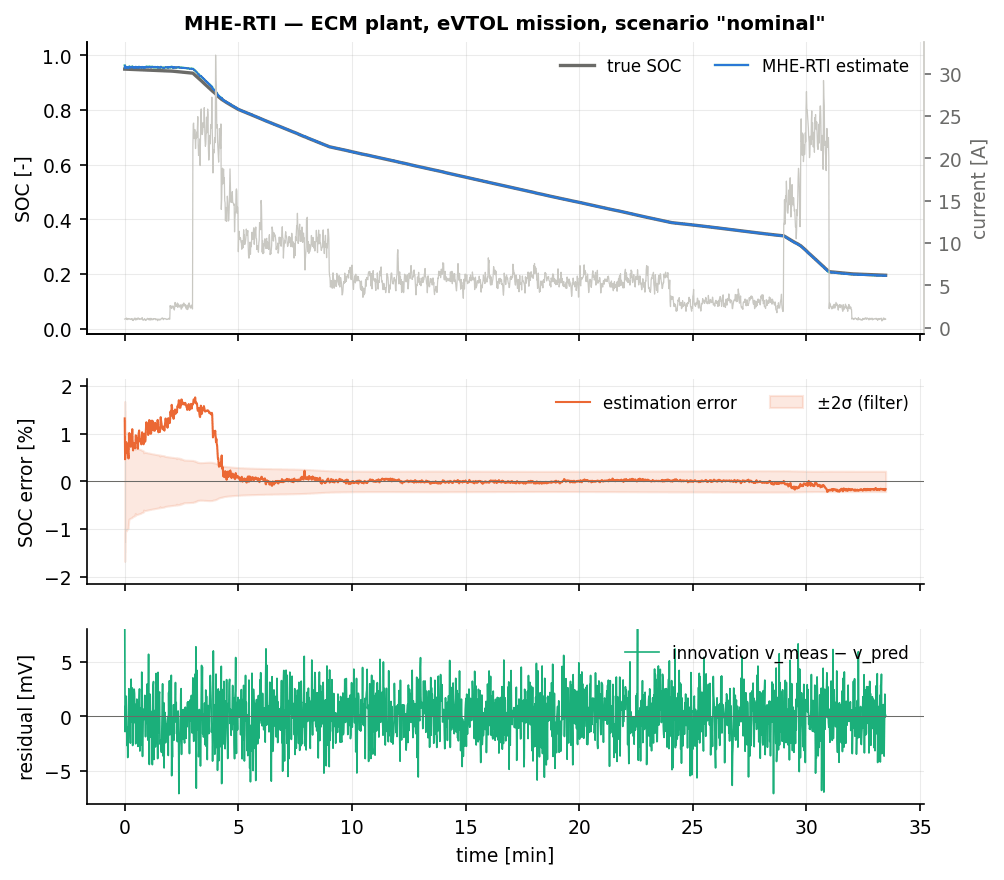
\includegraphics[width=\textwidth]{figures/cell_MHERTI_nominal.png}
\caption{MHE-RTI on the nominal eVTOL mission: true and estimated SOC (top), estimation error with
the $\pm2\sigma$ band from $\mD_N^{-1}$ (middle), voltage residual (bottom).}
\end{figure}
\begin{figure}[H]\centering
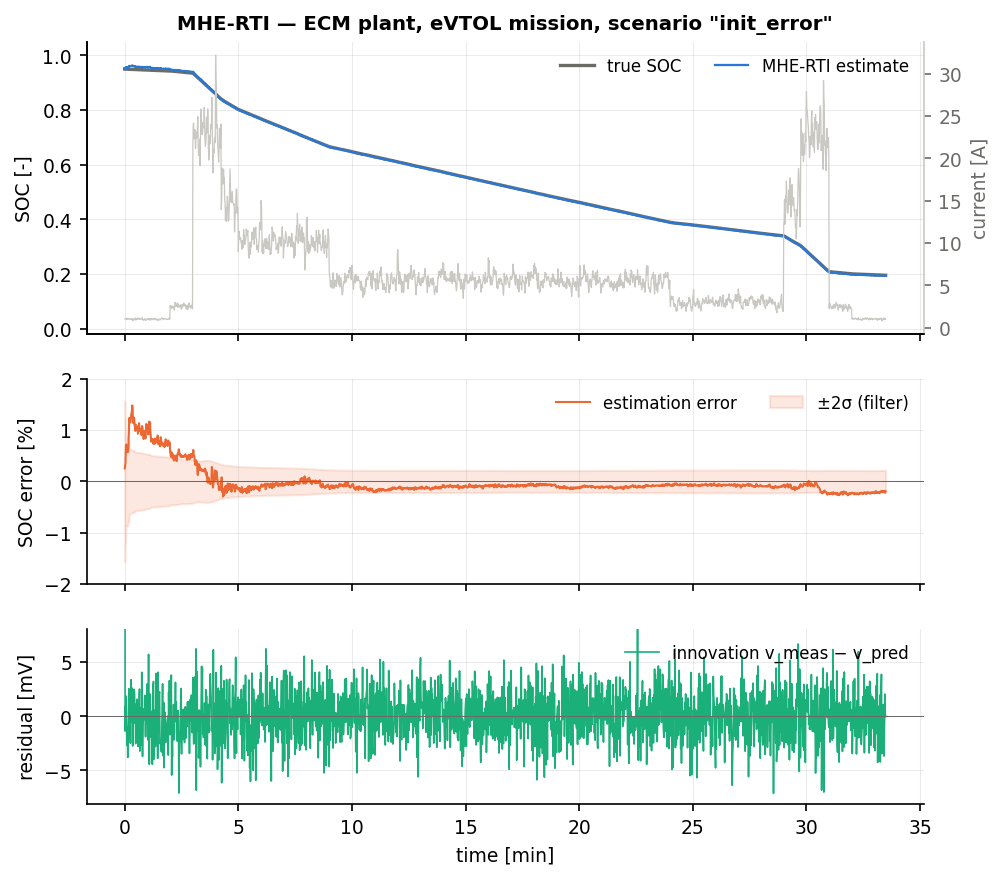
\includegraphics[width=\textwidth]{figures/cell_MHERTI_init_error.png}
\caption{MHE-RTI with a \SI{35}{\percent} initial SOC error.  One Gauss--Newton step per sample,
warm-started by the shift \cref{eq:rti-shift}, removes the transient within the first sample.}
\end{figure}

All numbers below are three-seed means in per cent SOC from Table~\ref{tab:cell_MHERTI}.

\paragraph{Acceptance.}  $\mathrm{rmse}/\mathrm{rmse_{ss}} = 0.36/\SI{0.08}{\percent}$ on
\texttt{nominal} and $0.23/\SI{0.11}{\percent}$ on \texttt{init\_error}, with
$t_\text{conv} = \SI{0}{\second}$ and no divergence in any scenario or seed.  The steady-state
error is within a factor of two of the EKF's \SI{0.05}{\percent} --- and slightly \emph{better}
than the converged variant of Chapter~\ref{ch:mhe} (\SI{0.11}{\percent}), which is the first
indication of the pattern that runs through this whole section.

\paragraph{One iteration versus five.}  This is the measurement the chapter exists for
(steady-state SOC RMSE [\si{\percent}], three-seed means):
\begin{center}
\begin{tabular}{@{}lcccccccc@{}}
\toprule
& \texttt{nom.} & \texttt{init} & \texttt{outl.} & \texttt{c.bias} & \texttt{aged} & \texttt{drop.} &
\texttt{comb.} & \si{\micro\second}/step \\
\midrule
EKF                      & 0.05 & 0.05 & \textbf{0.21} & 0.61 & 1.52 & 0.46 & 12.44 & \phantom{0}0.48 \\
\texttt{MHE-RTI} (1 it.) & 0.08 & 0.11 & 0.70 & \textbf{0.10} & \textbf{0.71} & 0.43 & \textbf{0.50} & 17.3 \\
\texttt{MHE} ($\le5$ it.)& 0.11 & 0.10 & 0.49 & 0.09 & 0.79 & \textbf{0.41} & 0.69 & 32.4 \\
\bottomrule
\end{tabular}
\end{center}
Across the eleven ECM scenarios the two variants differ by less than \SI{0.1}{\percent} SOC on
\emph{eight} of them, while the converged estimator costs exactly \textbf{1.9} times as much.  The
exceptions are informative rather than large: the converged solver is \SI{30}{\percent} better on
\texttt{outliers} ($0.49$ vs.\ $0.70$), where re-linearising repeatedly lets the window redistribute
a \SI{50}{\milli\volt} spike more evenly, and the real-time iteration is \SI{28}{\percent} better on
\texttt{combined} ($0.50$ vs.\ $0.69$), \SI{10}{\percent} better on \texttt{aged\_cell} and
\SI{27}{\percent} better on \texttt{nominal}, where the one-step lag behaves like a small amount of
extra damping against a persistently drifting model.  \textbf{The real-time iteration delivers the
accuracy of the converged solver --- on several scenarios, slightly better than it --- at half the
cost and with a constant, data-independent execution time}, which is precisely the claim of
\citet{diehl2005rti} and \citet{kuhl2011rtimhe}, here confirmed on a battery-estimation problem.

\paragraph{The scenarios the method wins.}  \texttt{combined}: $0.74/\SI{0.50}{\percent}$ against
the EKF's $16.02/\SI{12.44}{\percent}$, a factor of \textbf{25} in steady-state error, and
$t_\text{conv} = \SI{0}{\second}$ against the EKF's failure to converge at all.
\texttt{current\_bias}: $0.54/\SI{0.10}{\percent}$ against $0.54/\SI{0.61}{\percent}$, a factor of
\textbf{6}, from the horizon's ability to distinguish a slowly integrating sensor bias from a state
error.  \texttt{aged\_cell}: $1.20/\SI{0.71}{\percent}$ against $1.18/\SI{1.52}{\percent}$, a factor
of $2.1$.  All three are state-equation errors, which is what a window is good for.  What
\cref{eq:rti-fixed} adds is the reassurance that a single iteration loses nothing on them ---
\SI{0.50}{} against the converged \SI{0.69}{\percent} on \texttt{combined} --- because the
per-sample perturbation $\Delta_k$ stays small even when the total error is large.

\paragraph{Other scenarios.}  On \texttt{sensor\_dropout} the estimator gives
$1.51/\SI{0.43}{\percent}$ against the EKF's $0.72/\SI{0.46}{\percent}$: the peak excursion during
the \SI{15}{\second} fault is \SI{6.7}{\percent}, three times the EKF's, but the recovery is much
cleaner and the box constraint keeps every node feasible throughout.  On \texttt{hot} it gives
$0.23/0.04$, matching the EKF; on \texttt{preisach} $0.97/0.46$ against $0.58/0.20$.  Against
these, \texttt{noise\_step} ($0.99/1.23$ against $0.18/0.12$) and \texttt{cold} ($0.75/0.76$
against $0.20/0.16$) are clearly worse, for the arrival-cost reason analysed in
Chapter~\ref{ch:mhe}; the statistically consistent arrival mean recovers \SI{0.13}{} and
\SI{0.19}{\percent} on those two scenarios at the cost of \texttt{aged\_cell} and
\texttt{combined}.  \texttt{param\_mismatch} $2.40/\SI{2.19}{\percent}$ is the worst ECM row of the
sweep (EKF $1.28/1.36$): a \SI{30}{\percent} error in $R_0$ is a model error that neither a longer
horizon nor more iterations can fix, and the fading-memory arrival cost merely lets the estimate
chase it.  The online residual learner of Chapter~\ref{ch:elmrlsekf} is the right tool for that
failure mode, and combining the two --- an ELM residual inside the MHE cost --- is an obvious and
unexplored extension.

\paragraph{Electrochemical (SPM) plant.}
\begin{figure}[H]\centering
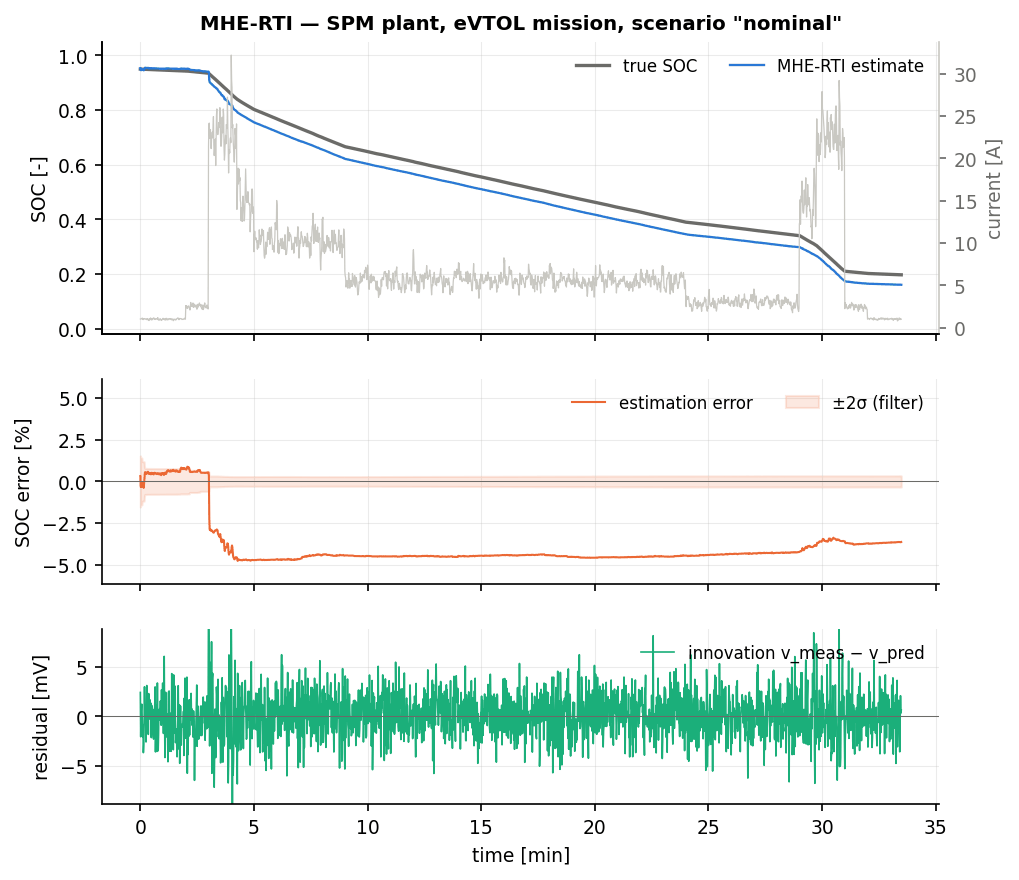
\includegraphics[width=\textwidth]{figures/cellspm_MHERTI_nominal.png}
\caption{MHE-RTI on the SPM plant, nominal eVTOL mission.  Twenty-one measurements all carrying the
same \SI{4}{\milli\volt} model bias look like a displaced state, and the least-squares fit
displaces it.}
\end{figure}
On the electrochemical plant the estimator gives \SI{4.55}{\percent} on \texttt{nominal} against
the EKF's \SI{3.73}{\percent} and the converged variant's \SI{3.45}{\percent}, and it beats the EKF
on only two of the nine SPM scenarios (\texttt{cold} $5.75$ vs.\ $7.35$, \texttt{param\_mismatch}
$3.00$ vs.\ $3.13$).  \Cref{sec:mhe-results} of Chapter~\ref{ch:mhe} analyses why in full; the
short version is that \cref{eq:mhe-nlp} assumes the model is right up to zero-mean noise, and a
structured \SI{4}{\milli\volt} output bias is indistinguishable, over a two-second window, from a
state displacement.  Two observations are specific to the real-time iteration.  First, the ranking
between the two MHE variants \emph{reverses} here: the converged solver is \SI{24}{\percent} better
on \texttt{nominal} (\SI{3.45}{} against \SI{4.55}{\percent}) and better on six of the nine SPM
rows, because with a biased model the warm start is no longer close to the optimum --- the solution
manifold that \cref{eq:rti-fixed} assumes the iterate tracks is itself being pushed away by an
error the model cannot represent, so $\Delta_k$ is no longer small and one iteration no longer
suffices.  \textbf{The real-time iteration's cost/accuracy bargain is contingent on the model being
approximately right}; that is a useful thing to know about it, and it is invisible on the ECM
plant, where the bargain looks free.  Second, the worst SPM rows are \texttt{noise\_step}
(\SI{7.82}{\percent}) and \texttt{sensor\_dropout} (\SI{7.65}{\percent}), both cases in which the
smoothing arrival cost recycles data that is either noisier or more wrong than $\mR$ declares ---
the same weakness as on the ECM plant, amplified.  None of this touches the ECM results: the
\texttt{current\_bias} (\SI{0.10}{\percent}) and \texttt{combined} (\SI{0.50}{\percent}) figures
stand, and \texttt{combined} remains the best result in this report on that scenario, ahead of the
fixed-interval URTS smoother (\SI{0.67}{\percent}) and of the converged MHE.

\paragraph{Cost in context.}  \SI{17.3}{\micro\second} per sample is $36\times$ an EKF and
\SI{0.017}{\percent} of a \SI{100}{\milli\second} sampling period.  For a single cell that is
irrelevant; for a \num{100}-cell pack sampled at \SI{10}{\hertz} it is \SI{1.7}{\milli\second} of
every \SI{100}{\milli\second}, which is affordable but no longer free, and argues for the
architecture in which MHE runs on a small number of representative or suspect cells while the rest
are tracked by EKFs.

\section{Summary}
MHE-RTI performs exactly one Gauss--Newton iteration of the constrained moving-horizon problem per
sample, warm-started by shifting the previous window's solution and appending one model step.  The
contraction argument \cref{eq:rti-fixed} bounds the resulting tracking error by
$\kappa/(1-\kappa)$ times the per-sample displacement of the solution manifold, which for a
\SI{10}{\hertz} battery model is tiny --- and the benchmark confirms it: on the ECM plant the
single-iteration estimator matches the converged one on eight of eleven scenarios and beats it on
\texttt{nominal}, \texttt{aged\_cell} and \texttt{combined}, at half the cost and with a constant,
data-independent execution time.  It is the best estimator in this report on \texttt{combined}
(\SI{0.50}{\percent} where the EKF has \SI{12.44}{\percent} and never converges) and second only to
its own converged variant on \texttt{current\_bias} (\SI{0.10}{\percent} against the EKF's
\SI{0.61}{\percent}).  It is worse than the EKF
wherever the sensor noise exceeds what $\mR$ declares, it cannot repair a parameter error, and on
the electrochemical plant --- where the output equation carries a structured \SI{4}{\milli\volt}
bias --- the bargain breaks down: the warm start is no longer near the optimum, the converged
variant recovers \SI{24}{\percent}, and both lose to a plain fading-memory EKF.  Use it as the
default moving-horizon estimator whenever the model is approximately right; when it is not, pay for
the iterations, or fix the model.
